% slides.tex — Ruben: 60s pitch deck (3 slides)
\documentclass[aspectratio=169,14pt]{beamer}
\usetheme{default}
\usecolortheme{orchid}

\usepackage[utf8]{inputenc}
\usepackage[T1]{fontenc}
\usepackage{tikz}
\usetikzlibrary{arrows.meta,positioning,shapes.geometric}

% Clean look
\setbeamertemplate{navigation symbols}{}
\setbeamertemplate{footline}{}
\setbeamercolor{frametitle}{fg=white,bg=purple!80!black}
\setbeamercolor{block title}{bg=purple!70!black,fg=white}
\setbeamercolor{block body}{bg=purple!5}
\setbeamercolor{itemize item}{fg=purple!80!black}
\setbeamertemplate{itemize item}{\raisebox{0.15ex}{\small$\blacktriangleright$}}

\title{Ruben}
\author{David Korcak \quad Frantisek Kmjec}
\date{Hack-Nation 2026}

\begin{document}

% ── Slide 1: Title + What ───────────────────────────── (~15s)
{
\setbeamercolor{background canvas}{bg=purple!80!black}
\begin{frame}[plain]
\vfill
\centering
{\Huge\bfseries\color{white} Ruben}\\[10pt]
{\large\color{white!80} Turn photos, videos, text, and audio\\into music you can understand and control.}\\[18pt]
{\color{white!60}\normalsize Multimodal $\to$ Semantic Tree $\to$ Music}\\[8pt]
{\color{white!50}\small David Korcak \quad Frantisek Kmjec \enspace$\cdot$\enspace Hack-Nation 2026}
\vfill
\end{frame}
}

% ── Slide 2: How It Works ────────────────────────────── (~30s)
\begin{frame}{How Ruben Works}
\centering
\vspace{-1mm}
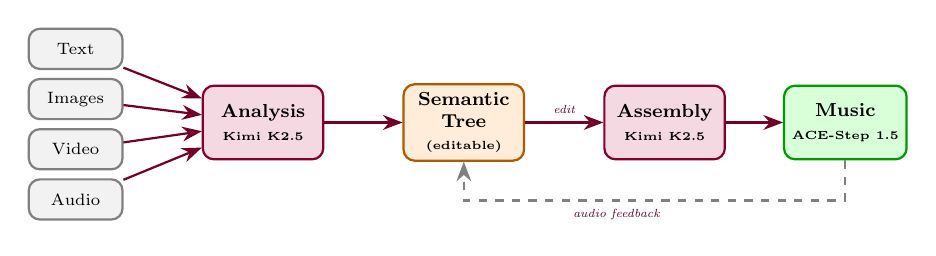
\begin{tikzpicture}[scale=0.85, every node/.style={transform shape},
  stage/.style={draw=purple!70!black, thick, rounded corners, fill=purple!10, minimum width=18mm, minimum height=11mm, align=center, font=\footnotesize\bfseries},
  input/.style={draw=gray, thick, rounded corners, fill=gray!10, minimum width=14mm, minimum height=6mm, align=center, font=\scriptsize},
  arr/.style={-{Stealth[length=2.5mm]}, thick, purple!60!black},
  label/.style={font=\tiny\itshape, purple!50!black}
]
% Inputs stacked
\node[input] (text) at (-4,0.9)  {Text};
\node[input] (img)  at (-4,0.15) {Images};
\node[input] (vid)  at (-4,-0.6) {Video};
\node[input] (aud)  at (-4,-1.35){Audio};

% Pass 1
\node[stage, fill=purple!15] (pass1) at (-1.2,-0.2) {Analysis\\{\tiny Kimi K2.5}};

% Tree
\node[stage, fill=orange!15, draw=orange!70!black] (tree) at (1.8,-0.2) {Semantic\\Tree\\{\tiny(editable)}};

% Pass 2
\node[stage, fill=purple!15] (pass2) at (4.8,-0.2) {Assembly\\{\tiny Kimi K2.5}};

% Output
\node[stage, fill=green!15, draw=green!60!black] (music) at (7.5,-0.2) {Music\\{\tiny ACE-Step 1.5}};

% Arrows
\foreach \n in {text,img,vid,aud} \draw[arr] (\n) -- (pass1);
\draw[arr] (pass1) -- (tree);
\draw[arr] (tree) -- node[above, label] {edit} (pass2);
\draw[arr] (pass2) -- (music);

% Feedback
\draw[arr, dashed, gray] (music.south) -- ++(0,-0.6) -| node[below, pos=0.3, label] {audio feedback} (tree.south);
\end{tikzpicture}

\vspace{3mm}
\begin{columns}[T]
\column{0.3\textwidth}\centering
\textbf{Pass 1: Decompose}\\
{\small LLM builds a tree of\\musical characteristics}
\column{0.3\textwidth}\centering
\textbf{Edit the Tree}\\
{\small Tweak any node —\\mood, instruments, tempo}
\column{0.3\textwidth}\centering
\textbf{Pass 2: Assemble}\\
{\small LLM resolves conflicts\\into a coherent prompt}
\end{columns}
\end{frame}

% ── Slide 3: Closing ─────────────────────────────────── (~15s)
{
\setbeamercolor{background canvas}{bg=purple!80!black}
\begin{frame}[plain]
\vfill
\centering
{\Huge\bfseries\color{white} Ruben}\\[14pt]
{\large\color{white!80} Interpretable \enspace$\cdot$\enspace Editable \enspace$\cdot$\enspace Multimodal}\\[18pt]
{\color{white!65}\normalsize
Style transfer via text \enspace$\cdot$\enspace Version history \enspace$\cdot$\enspace Full parameter control}\\[14pt]
{\color{white!50}\small Kimi K2.5 \enspace$\cdot$\enspace ACE-Step 1.5 \enspace$\cdot$\enspace React + FastAPI}
\vfill
\end{frame}
}

\end{document}
